\documentclass[../../thesis.tex]{subfiles}
\graphicspath{{\subfix{diagrams/}}}

\begin{document}
The goal of the work is to explore if zk-rollups can be used to aggregate Uniswap trades in an effective manner. The prototype is able to aggregate trades for a single trading pair, Ether and an ERC-20 token of choice. First, we'll look at the systems design to understand how the different entities work together.


The system consists of two main entites that are required for it to function. The first entity to look at, is the on-chain entity, we call zkSwap. zkSwap is a smart-contract deployed on the Ethereum blockchain and has three main jobs, verifying deposit and withdraw batches, processing instant withdraws and verifying trade batches. It holds users funds and exposes the on-chain functionality, to the user and emits balance updates. 

The second entity to look at is the aggregator. The aggregator consists numerous systems, both off-chain and on-chain, and is mainly tasked with receiving deposits, withdraws or trade orders, aggregating and executing them, and then verifying them with the zkSwap contract. The aggregator stores a merkle-tree of users balances and keeps it in sync by listening for event emitted by the zkSwap contract.

\begin{figure}[h]
    \centerline{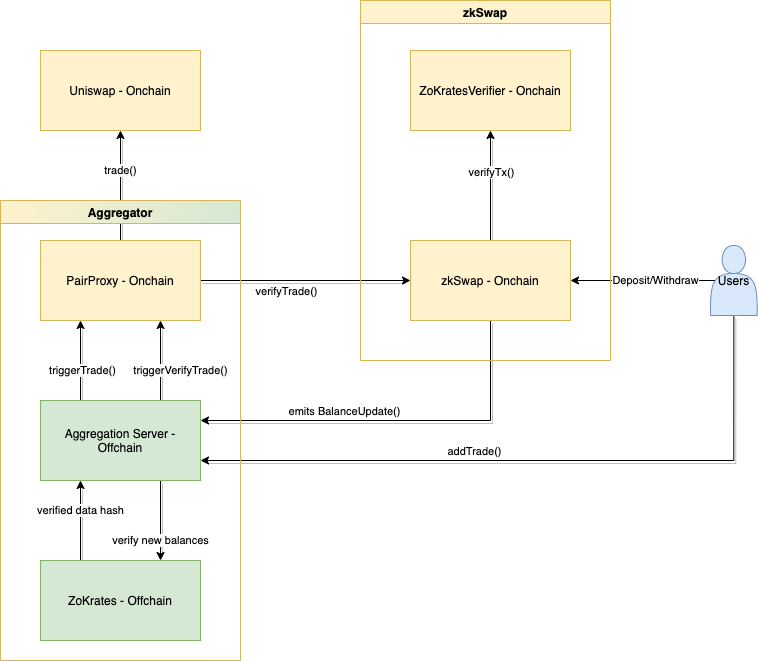
\includegraphics[totalheight=8cm]{diagrams/architecture.png}}
    \caption{High level architecture of the system}
    \label{fig:architecture}
\end{figure}

\subsection{Design}
In this section we will explore the design of the system, looking at the different functionalities and dependencies to understand the core mechanics of how the different entities interact with each other. 

The two main entities of this system are the zkSwap smart contract and the aggragator. 


\subsubsection{zkSwap Smart-contract}
The zkSwap contract, is the core entity the user interacts with. Its a smart-contract, that from the users perspective, is mainly used for depositing and withdrawing funds in out system and keeping track of user balances.

\paragraph{Deposits}
To use the system a user first has to deposit funds into the smart-contract. The funds need to be sent as a normal on-chain transaction to the smart-contract, where they will be stored, while the balance is then represented in layer-2. To deposit funds, a user calls the deposit function in the zkSwap smart-contract and adds the funds to be deposited to the transaction. When the funds have been received, an event is emited informing the aggregator about the new deposit. At the same time, the user signs the deposit data, and sends it to the aggregator as a message. The aggregator aggregates a number of deposits, verifies the correctness in the zkSwap smart-contract, at which point they will show up as balance for the user.

\paragraph{Withdraws}
When withdrawing funds, the user needs to decide between an aggregated withdraw, similar to the deposit, or an instant on-chain withdraw. The aggregated withdraw works just like the deposit, only difference being the a withdraw amount is specified instead of sending funds. After the aggregation is complete, the user will receive the funds as an on-chain transaction. A user can also withdraw funds by using the instant withdraw feature. While it costs significantly more gas to withdraw funds with this function, it can be used without the aggregator being online. The protects the user from not being able to withdraw its funds in case the aggregator is offline or has turned malicious. 

\paragraph{Verification of Aggregated Trades}
The last main functionality of the zkSwap contract is the verification of aggregated trades. Once the aggregator has completed the aggregation batch, it send the new balances along with a zkSNARK proof and the traded funds to the zkSwap contract. If the proof is valid and the correct amount of funds have been sent to the zkSwap contract, the new balances are emitted, finanlizing the state. The aggregator is now refunded, receiving the funds it spent when executing the aggregated trade on Uniswap.

\subsubsection{Aggregator}
As the name implies, the aggregators job is aggregating deposits, withdraws and trades. It facilitates the aggregation of these operations and is built in a way that ensures correct execution, while no trust assumptions are made. The aggregator relies on a number of different systems to function, in the section we look at it from a functional perspective, explaining the core functionalities and what systems is relied on. This will be explained in the implementation section in more detail.

\paragraph{Deposits and Withdraws}
When a user deposits or withdraws funds, choosing the aggregated type, the user sends a signature of the deposit/withdraw operation to the aggregator. The aggregator receives theses messages, collecting them as the next aggregation batch. Once a number of messages have been received, the new balances are caluculated and passed to the corresponding ZoKrates program, where the correctness of the balances and signature is checked. If this is successful, a zkSNARK proof object is created. The aggregator now send the proof, along with the new balances to the zkSwap smart-contract. If the proof is valid, the new balances are emitted by the zkSwap contract. Each withdraw will now be credited by sending the requested funds to the users. 

\paragraph{Aggregating Trades}
A user can make a trade by sending a message to the aggregator. Similarly to deposits and withdraws, the aggregator collects messages as the next aggregation batch. All received trade messages are now aggregated and offset internally, resulting in the 'net-trade' that must be executed to honor all trades of the batch. The 'net-trade' is then sent to the 'PairProxy' smart-contract as a on-chain transaction, which in turn will execute it on Uniswap. The details and reasoning of this contract will be explained in the implementation section. Once the trade is executed, the new balances are calculated and the correctness ensured by using the corresponding ZoKrates program. The resulting proof and the new balances are sent to the PairProxy smart-contract. The previously purchased funds are now added to the transaction, forwarding it to the zkSwap smart-contract. The proof is verified, the new balances emitted, and the aggregator is refunded the amount paid in the 'net-trade'. 

\paragraph{Storing Balances in a Merkle Tree}
The aggregator keeps track of the balances by listening to events emitted by the zkSwap smart-contract. When an event is received, the balance is either updated or added to the merkle tree if its a new user. Since the events stay on-chain, the merkle tree can always be rebuilt by querying these events, and updating the merkle tree sequentually. The aggregator provides endpoints where balances can be queried, along with the corresponding merkle paths, which are used throughout the system. It is important to remember, that the balances are public and can be queried by anyone.

\paragraph{PairProxy Smart-contract}
This smart-contract is controlled by the aggregator and is used to execute trades on Uniswap and forward transactions to the zkSwap smart-contract. The aggregator can use it to hold funds, which makes the transactions cheaper. 


\subsection{Implementation}
In this section we will look at the way these fuctionalities are implemented and how they function. 

\subsubsection{Storing and Updating Balances} \label{balances}
Balances are represented as a balance object in our system. This object consists of four fields that are neccecary to represent balances correctly, the ethAmount, the tokenAmount, the users address and a nonce. It is important to understand the core technique used to store and update balance objects before we look at the different functions that trigger them. We want to make balance object updates as cheap as possible, while not relying on any external data availability. Essentially, this means that we need to store the balances on-chain. Storing data on-chain is typically very expensive. It is important to make a distinction between storing data in a smart-contracts runtime and storing data in the event log. Both methods of storage are on-chain, using the event log is significantly cheaper though. A disadvantage of using the event log however, is the fact that it can't be accessed from a smart-contracts runtime, and must be queried by a client. This solves the external data availablity problem. We can store balances cheaply by emitting the `BalanceUpdate' event, without relying on other systems to stay online. A client can query the event log, gather the required data and pass it as parameters to the transaction. However, we now need a mechansism to ensure, the user is passing correct data. 

\paragraph{Merkle Trees}
We can achive this, be using a merkle tree \cite{szydlo2004merkle}. Merkle trees are a suitable data structure, as the merkle root represents the entire tree state in a highly compressed form, while proving a leafs inclusion in the tree can be done with O(log n). This is ideal for our use-case. Every balance is stored as a leaf in a merkle tree, running in layer-2. The merkle tree is built and kept in sync by subscribing to the ‘BalanceUpdate’ event emitted by our smart-contract. A client can query balances from this  tree, receiving the valid merkle path along with the balance object. The correctness of that data can be proven by recreating the merkle root, which is stored and updated in the zkSwap smart-contract. Since all changes in balance are committed by emitting the `BalanceUpdate' event, it must be ensured that merkle root is changed according to the updated balance. It is important to understand, that the only way balances can be updated is with the `BalanceUpdate' event.

\subsubsection{Aggregating Balance Updates} \label{aggr_balance}
Updating a users balance is at the core of this system. Deposits results in a balance update, as do trades and withdraws. Before looking at these in detail, it is important to understand how balance updates can be aggregated, reducing the transaction costs for these operations. Since balances are stored in a merkle tree, we can ensure the correctness of a balance by running an inclusion proof. However, running this in a smart-contract is expensive, as a lot of hashing is required. To reduce this cost, we can ensure the correctness by running this in a ZoKrates progam. If the ZoKrates program exits successfully, a zkSNARK proof is generated, which can be used to verify our execution on-chain.

\paragraph{Merkle Inclusion Proofs}
In order to ensure the correctness of balance updates, we first need to verify the inclusion of the balances involed in the merkle tree. Doing this one by one is simple. Every balance provides its merkle path which it can be hashed with. If the resulting hash matches the current merkle root stored in the zkSwap smart-contract, we can be assured the provided balance is included in the tree. At the same time, this enables us to reuse the merkle path for updating the balance. We can simply change the balances values after passing the inclusion proof, rehash with the merkle path, and the result is the correct root for the updated balance leaf. Since the majority of hashing is done in ZoKrates programs, looking for a hashing function that can efficiently be executed in a zkSNARK circuit is important. At the same time, we also want the hashing function to be somewhat affordable when executing in the smart-contract. In this implementation we will utilize the MiMC \cite{albrecht2016mimc} hashing function, as it can used in zkSNARK circuits efficiently. The MiMC function is used with the feistel structure and setup with 220 rounds, which is deemed secure. The merkle tree is hashed with the MiMC hashing algorithm. 

\paragraph{Chaining Inclusion Proofs} \label{chain_inclusion}
When dealing with multiple balances, the inclusion proof can be done the same way. Every balance provides its merkle path, the resulting hashes should be the same for each balance. Things become more difficult when updating the balances. Updating the first balance in the batch now invalidates the merkle path of all following balances. In order for this to work, the merkle paths for each balance must be created sequetually. This can be solved by sorting the balances before hand, and generating each merkle path based on the changes of the previous balance. The new root of the first balance is the old root of the next balance. This can be chained to an infite length and results in a constant number of hashes required for each balance update. The last hash to be computed is the new merkle root, representing all balance updates.

(Add Algo here)

\paragraph{Authorizing Balance Updates}
We still need to ensure the user has authorized this balance update though. As balance updates are emitted as an event, anyone can access them and compute valid merkle paths for any balance in our system. The data is public. This would, for example, allow any user to withdraw any balance. To ensure a user is authorized to update a balance, we need ensure the user controlls the private key belonging to the balances user address. This can be achived by requesting a signature from the user. However, it must be remembered, that this signature must also be verifiable in our ZoKrates programm, which is unable to utilize the secp256k1 curve, used for signing Ethereum transaction, efficiently \cite{deml_2019}. For that reason the Baby JubJub curve is used in combination with the EdDSA signature scheme, which can be run more efficiently in a ZoKrates program. The user submits a signature containing the current merkle root and the update message. This ensures three things. It proves the user controlls the private key belonging the the balance objects address, thereby authorizing the order. We also make sure, the balance update corresponds to the amount signed by the user, ensuring the transition is done correctly. By signing the current merkle root, we make sure, that the signature can't be reused in a replay attack. For instance, the aggregator could decide to store these signatures secretly, and reuse them without the users consent if this was omitted. By checking if the current root is equal to the signed root when verifying the zkSNARK proof, we prevent replay attacks. It is important to note, that different programs are used for deposits/withdraws and trade aggregation. As already mentioned, these programs have a number of checks that ensure the changes in balance correspond to the values specified in the signed update message. These will be explained in the respective sections. 

\paragraph{Creating a EdDSA Signature}
At the time of writing, metamask does not support signing with the EdDSA signature scheme on the Baby JubJub curve. Fortunetly, we can derive a Baby JubJub private key from an EcDSA signature, and then use the derived key to sign with the EdDSA signature scheme over the Baby JubJub curve. This signature can then be verified cheaply in a zkSNARK circuit. It must also be mentioned, that we utilize the MiMC hashing function to hash the message, as its efficient to run in a zkSNARK circuit. \todo{explain situation with hermez}

\paragraph{Executing and Reducing On-chain Verification Costs} \label{exec_and_reduce}
All of these checks are performed as a ZoKrates program. If no checks fail, the proof can now be generated.  We have now successfully verified the new balances, and we could use these values to generate the proof, which will then be used to verify everything on-chain. When verifying the ZoKrates program on-chain, each output of the program is part of the proof object, adding an iteration to the proving logic. The amount of outputs the ZoKrates program has, influences the verifications costs. We can reduce this cost by returning a hash of the resulting data, thereby reducing the amount of outputs. Since the aggregator computed the balances in the first place, and the ZoKrates program only verified the updates, the aggregator can pass that data as part of the verify transaction, but excluded from the ZoKrates proof object. By hashing the data with the SHA256 hashing algorithm in the zkSwap smart-contract, we can ensure that data correctness by comparing it to the hash that is part of the proof object. As a result, the ZoKrates program only returns this hash as an output value, which we call the data hash. While the SHA256 hashing algorithm is inefficient to run in zkSNARK, and its very cheap use in a smart-contract. Since every balance update in an aggregation batch needs to be hashed on-chain, reducing the on-chain cost is more favorable, compared to reducing the complexity of the zkSNARK program. 

\subsubsection{Deposit}
When using the system, a user first has to deposit funds. Since the entire idea of zk-rollup is to move funds to layer-2, the deposit function can be seen as a bridge that connects the mainnet and layer-2. When a user makes a deposit, the funds are represented as a balance object in layer-2, which in turn gives custody to these funds. When moving funds in layer-2, we don't actually move the funds residing in the smart-contract, but update the balance objects to represent the movement and verify that movement for correctness with a zkSNARK proof\todo{Maybe remove this?}. Since a balance object gives a user custody of represented funds, it can always be redeemed, moving from layer-2 back to mainnet.  

\paragraph{Movement of Funds}
To move funds to layer-2, a user first needs to send the funds to the zkSwap smart-contract. This is done by calling the deposit function in the zkSwap smart-contract and attaching the funds to the transaction. The deposit function now emits a `Deposit' event, containing the type of fund (Ether or ERC20), the amount and the address of the user making the deposit. This event notifies the aggregator of the deposit and ensures the user has actually deposited a certain amount of funds. This is the first step of the deposit.

\paragraph{Aggregating Deposits}
After the funds have been sent to the smart-contract, the user creates a signature containing the type of aggregation (deposit/with), the changes in Ether and token balance, the users address and the current merkle root. This signature is sent to the aggregator as an HTTP request. The aggregator checks the signature of each incoming request and makes sure a matching `Deposit' event has been emitted. This ensures the user has actually sent funds to the smart-contract. After a number of deposits have been received, the aggregation is started. The aggregator now generates a `BalanceMovementObject' for each deposit, containing the old balance, the new balance, the merkle path and the signature. This is passed to the `ProcessBalanceMovement' ZoKrates program, along with the current merkle root. As explained in S. \ref{chain_inclusion}, the inclusion proof is now performed on the old balance. If the old balance is included in the merkle tree, the signature is checked, along with the change of balance. The signed amount should equal the added amount in the new balance, the nonce must be incremented and the address the same. If these checks pass, we calculate the new new merkle root, by rehashing the new balance with the merkle path. We do this for each `BalanceMovementObject', and hash the new balances, as explained in S. \ref{exec_and_reduce}, along with the old merkle root and the new merkle root, to reduce the on chain verification costs. This results in the data hash. 

\paragraph{Verifying Deposits On-chain}
Once the ZoKrates program has run successfully, the proof can be generated, which is used for verification in the zkSwap smart-contract. The aggregator calls the `verfiyBalanceMovement' function in the zkSwap smart-contract and attatched the proof, along with the new balances and the old and new merkle root to the transaction. As a first step, the balances and roots are hashed, and the result of the hash compared to the output field in the ZoKrates proof object. If these hashes match, we can be assured, the the aggregator has attatched the data that has been checked by the ZoKrates program. Next, we check if the old root, matches the current root stored in the zkSwap smart-contract. This ensures that a generated proof can't be reused in replay attacks. As a last check, the ZoKrates proof object is checked with the verifier smart-contract deployed for this purpose. If this is also successful, we have proven, that the aggregator has proccessed the deposits correctly. We now iterativly emit the new balance objects with the `BalanceUpdate' event, and update the merkle root in the smart-contract. The deposits have now been processed and show up as balance for the users. 

\subsubsection{Aggregated Withdraws} \label{with}
The aggregated withdraws largly follow the logic of the deposits, so only the core differences will be explained here. Instead of sending funds to the zkSwap smart-contract, we are requesting them. Since the user already has a balance in the system, we don't need to notify the aggregator about the amount a user wants to withdraw, which in turn means we don't need an on-chain transaction to trigger the withdraw. A user creates a signature of its address, the current merkle root, type of funds and the amount to be withdrawn, and sends it to the aggregator as an HTTP request. Once the aggregation starts, the aggregator checks the users signature, and ensures that the users balance covers the withdraw. Just like with deposits, a `BalanceMovementObject' is created, the type being set to withdraw. The withdraws are verified along with the deposits in the same ZoKrates program. This results in only one on-chain verification, which reduces verification costs. The `ProcessBalanceMovement' checks signature, the balances and if the the balance update corresponds to the amount signed by the user. On top of hashing the new balances, a withdraw object is also hashed, containing the type of funds and the amount. When verifying withdraws, along with the deposits, the withdraw objects will be used to send the funds from the smart-contract to the users. The new balances are emitted and the root updated. 

\subsubsection{Instant Withdraws}
A user also has the option to withdraw instantly, without being dependant on the aggregator. This ensures a user can always withdraw funds, even when the aggregator is failing or offline. Instead of sending the withdraw request to the aggregator, the withdraw is processed completly on-chain. The user attaches its balance object, along with the corresponding merkle path and the withdraw amount and fund type (Ether/ERC20) to the transaction. As a first step, the merkle inclusion proof is performed. The balance object is hashed, sequeutually with the merkle path. The resulting hash now equals the the merkle root stored in the zkSwap smart-contract if the correct balance object and merkle path have been submitted. It is checked if the balance can cover the withdraw, if thats the case the nonce is incremented, the new balance is calculated, and the new balance object hashed again. The new root is now computed by hashing with the merkle path, and updated in the smart-contract. The funds are now sent to the user and the new balance is emitted. It must be reiterated, that this is done completly on-chain and doesn't require the aggregator to be online. However, the gas costs of this transaction are significant, as hashing with the MiMC hashing algorithm is expensive in a smart-contract.

\paragraph{Authorizing Instant Withdraws}
This however, is an incomplete explaination, as we're not checking if a user is permitted to withdraw funds. As balance objects are emitted as an event, anyone can access them and compute valid merkle paths for any balance. This would allow any user to withdraw any balance. To ensure a user is permitted to update a balance object, we need ensure the user controlls the private key belonging to the balance objects user address. Fortunetly, we can ensure this by accessing the sender in transaction object. The Ethereum blockchain ensures a user is allowed to make a transaction by requiering the transaction to be signed with the private key of the senders address. If that signature is valid, it is proven that the user has access to the addresses private key and the transaction can be executed. Because of this, the transactions object sender can be trusted to be in controll of the corresponding private key. Instead of passing the users address as part of the balance object, the smart-contract uses the sender of the transaction object. This suffices as a security check.


\begin{figure}[h]
    \centerline{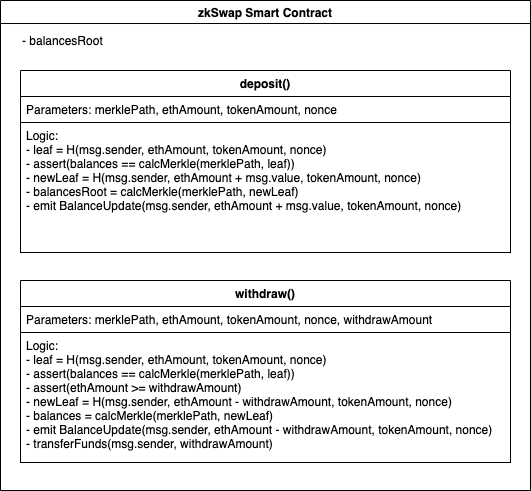
\includegraphics[totalheight=8cm]{diagrams/deposit.png}}
    \caption{Pseudocode of the deposit and withdraw steps}
    \label{fig:dep_with}
\end{figure}

\subsubsection{Aggregating Trades}
Before explaining the life-cycle of a trade aggregation batch, it makes sense to understand the mechanism that ensures the correct price of trades in an aggregation batch. After, we will go through the entire life-cycle of an aggregation batch, starting with a user adding a trade. 

\paragraph{Ensuring Correct Pricing}
The price between assets is constantly changing. At the same time, trades are being collected for aggregation. This results in a delay between an user sending a trade order and the actual trade execution, during which the price of an asset can change. On top of that, network congestion on the Ethereum blockchain can cause fruther delays in the execution. A mechanism is needed to define a 'worst-case' price, that is defined before users add orders to the aggregation. Once the aggregation is complete, a user can be sure to having paid no worse then the 'worst-case' price.

Another thing to consider is the bid-ask spread that exists in a trading pair. A spread is the difference between the current bid and ask price for an asset, where the bid always has to be a lower price. Intuitivly, this makes sense, the spread should at least equal the cost of converting from one asset to the other. There are a number of other factors that influence the bid-ask spread for a Uniswap trading pair. In this context however, it is sufficient to know that a spread is expected in any trading pair. This complicates the mechanism to ensure a worst-case price. 

Buy and sell orders are off-set internally once the aggregation starts, which results in the `net trade'. Since we don't know what orders will be received in an aggregation batch, we're unable to predict if the `net-trade' will be a buy or sell order. Since we have a bid-ask spread, and we can not predict which direction our net trade will be, we need to define a price range that at least equals the current bid-ask spread. This would suffice to ensure a worst-case price for a net trade in either direction if executed immediatly.
As the aggregation is also adding a delay between defining the price range and executing the trade, the price range should be larger then the spread. For this reason the zkSwap smart-contract defines a minSell and maxBuy price, defining that range. If the price on Uniswap has moved out of that range, while the aggregation was in progress, the trade won't be executed and the aggregation canceled. This can be formalized in the following way: 

$$\forall A_o\in A: x_s \leq x_e \leq x_b$$


where:
\begin{description}
\item[$A$] is the current aggregation batch
\item[$A_o$] a trade order
\item[$x_e$] is the effective price 
\item[$x_s$] is the minSell price
\item[$x_b$] is the maxBuy price 
\end{description}

\begin{figure}[h]
    \centerline{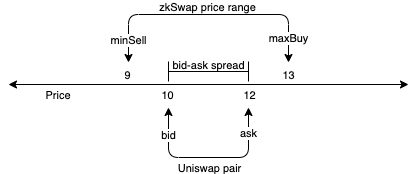
\includegraphics[totalheight=3cm]{diagrams/priceing.png}}
    \caption{Bid-ask spread and zkSwap price range}
    \label{fig:price}
\end{figure}

While this method ensures a 'worst-case' price for a trade, at the same time a maximum price is defined with it. Since we're matching buy and sell orders in one aggregation, there is no way around this. Once the aggregation is completed and verified on-chain, the new minSell and maxBuy prices are set, based on queried Uniswap prices, which are valid for the next aggregation batch.

\paragraph{Adding an Trade Order}
To make a trade, a user must create an trade object and sign it with its private key. The trade object consists of five fields that are needed to define the trade, the tradeDirection, deltaEth, deltaToken and the users address and current merkle root. Since ZoKrates only uses unsigned integers, we need the tradeDirection to calculate the new balance. Once signed, the trade object is sent to the aggregator as an HTTP request. As a first check, the aggregator checks if the signature is valid. This ensures, that the trade object was created by the someone in control of the addresses private key, thereby authorizing the trade order. The aggregator now queries the users balance from its merkle tree, and checks if the merkle root in the trade object is equal to the merkle root set in the zkSwap smart-contract. This ensures the signed trade object can't be reused in replay attacks. The aggregator also checks if the users balance can cover the trade, making sure enough balance has been deposited. A last thing to consider is ensuring the correct price of a trade. The aggregator checks if the implied price of the trade matches the ‘worst-case’ price stored in the zkSwap smart-contract. If all of these checks pass, the order is added to the trade pool, where it resides until the aggregation starts. It must be noted, that these checks are techniqually not needed to ensure the correctness of the aggregation, as the ZoKrates program performes the same checks. They are however needed, to prevent the aggregator from processing invalid trades, which would cause the ZoKrates program to exit in an error state, preventing the entire aggrgation. A trade is invalid, if it fails any of the checks described in this paragraph.

\paragraph{Executing Trade and Calculating New Balances}
At some point the trade aggregation is started. This could be triggered by a set blocknumber, the number of trade orders that have been received or any other useful condition defined by the aggregator. When aggregation is started, the first step is to calculate the `net trade'. Since our system aggregates buy and sell orders, we can offset those internally. By doing this, we're able to reduce the entire aggragation to one Uniswap trade, which saves gas. At the same time, we're saving on the 0.3\% liquidity provider fee, which is charged based on a trades volume. The net trade is the result of off-setting all trades in aggregation, buy or sell order, which results one side to equal zero. This trade is now sent as an on-chain transaction to the `PairProxy` contract, where the trade is now executed with Uniswap. The PairProxy contract is explained in detail in S. \ref{pairProxy}. 

The aggregator waits for the PairProxy smart-contract to emit the `TradeComplete' event, which will fire once the trade has been executed, containing the amount of assets aquired in the Uniswap trade. The amount received must at least imply the worth-case price, defined by the zkSwap smart-contract. In most situations, the implied price (effective price from here) will be better then the worst-case price. Based on the effective price, the users post-trade balances are calculated. For each trade, a `BalanceUpdateObject' is created, containing the old balance, the new balance, the merkle path and the signed trade object. The merkle paths for each `BalanceUpdateObject' are created as explained in S. \ref{chain_inclusion}. Now the `ProcessTrades' ZoKrates program is called, along with the `BalanceUpdateObjects', the current merkle root and the worst-case price.

\paragraph{Checking Pricing in ZoKrates}
We want to make sure that each trade has the same price, no matter if its a buy or sell order. It is also important that this price is no worse then the worst-case price, defined in the zkSwap smart-contract. We iterate through the `BalanceUpdateObjects', checking if each trade has the same price, and making sure it's greater or equal to the worst-case price. While doing this, we also calculate the `net-trade', which will represent the flow of funds between the zkSwap smart-contract and the aggregator. After this has completed, we are assured that each user is receiving a equal rate, at least matchig the worst-case price\footnote{The worst-case price will be compared to the one stored in the zkSwap smart-contract at a later stage, enforcing it for the entire aggregation.}, and we have calculated the `net-trade', which will be important when finalizing the aggregation.

\paragraph{Verifying Balances and Authorization in ZoKrates}
To ensure the correct aggregation of these trades, we still need to ensure the submitted old balances are part of the merkle tree and that the user has authorized the trade. While the aggregator has checked this already, it must be remembered, that the aggregator is an unstrusted party. We need to be able to verify the correct execution of these checks on-chain, which can be achived with zkSNARK. To ensure this, we largly folloe the steps described in S. \ref{aggr_balance}. We iterate through the `BalanceUpdateObjects' sequentially, checking if the merkle root can be recreated. If thats the case, we check if the signature is valid, and if the balance change matches the amounts specified in the trade object. Since the price hase been checked already, we're only checking the amounts here. Now we compute the new merkle root, based on the new balance. This root is then used to verify the balance of the next `BalanceUpdateObject', details of this are explained in S. \ref{chain_inclusion}. The last merkle root computed is the new merkle root, representing the entire merkle tree with the updated balances. 

\paragraph{Reducing On-chain Verification Costs in ZoKrates}
We have now successfully verified the new balances, and we could use these values to generate the proof, which will then be used to verify everything on-chain. As explained in S. \ref{exec_and_reduce} we can still reduce the gas needed for verifying the aggregation batch on-chain, by hashing the results, thereby removing them from the zkSNARK proof. As the last step of the ZoKrates program, we hash all new balances, the old and new merkle root, the net trade and the worst-case price. The resulting hash, called the data hash, is the only output of the ZoKrates program.


% When verifying the ZoKrates program on-chain, each output of the program is part of the proof object, adding an iteration to the proving logic. The amount of outputs the ZoKrates program has, influences the verifications costs. We can reduce this cost by returning a hash of the resulting data, thereby reducing the amount of outputs. Since the aggregator computed the balances in the first place, still holding that data, it can pass that data as part of the verify transaction, but excluded from the ZoKrates proof object. By hashing the data in the zkSwap smart contract, we can ensure that data correctness by comparing it to the hash that is part of the proof object. As a result, the ZoKrates program only returns this hash as an output value. While the SHA256 hashing algorithm is inefficient to compute in a zkSNARK program, it is cheap to execute in a smart-contract. Since this hashing must be performed for every trade aggregation and the amount of hashes grow linearly with the amount of trades in an aggregation, the SHA256 hashing algorithm us used. The new balances, old and new merkle root, the worst-case price and the net trade are hashed, resulting in what we call the data hash. 

\todo{Explain assumtions that can be made from proof in background, hashing as algo blaaa}

\begin{figure}[h]
    \centerline{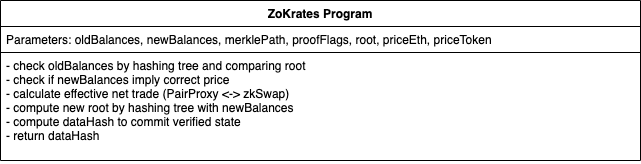
\includegraphics[totalheight=3cm]{diagrams/zokrates.png}}
    \caption{ZoKrates program checks}
    \label{fig:zokrates}
\end{figure}

\paragraph{Generating Proof and Verifying}
At this point the aggregator can start the proof generation of the ZoKrates program. This proof object is needed to verify the correct execution of our ZoKrates program as an on-chain transaction in the zkSwap smart-contract and includes, among other things, our data hash. To verify everything on-chain, and thereby updating balances of all balances involved in the aggregation, the proof object is passed, along with the new balances, the new merkle root and the net trade and sent to the PairProxy smart-contract. The `PairProxy' smart-contract receives the transaction, adds the funds previously traded with Uniswap to the transaction and forwards it to the `verifyTrades' function in the zkSwap smart-contract. 

\paragraph{Verifying the ZoKrates Proof}
The first thing checked in the zkSwap contract when receiving a trade aggregation batch, is the ZoKrates proof object. The verifier smart-contract is generated along with the the ZoKrates program, and can be used to verify the correct execution of that program using the proof object it generates. The verifier is called, along with the proof object passed as parameter. If the verifier return true, we have proven that our data hash was computed by running the `ProcessTrades' ZoKrates program, which in turn was used to generate the verifier. The remaining steps of the trade aggregation life-cycle happen in the zkSwap smart-contract, purely on-chain.

\paragraph{Recreating the DataHash and Ensuring Correct Price}
As a next check, we need to ensure that the aggregator has attatched the same data verified by the ZoKrates proof generation. This can be done by recreating the data hash. Just like the merkle root, this hash commits a certain state, which we can verify at a later stage. By using the properties of zkSNARK, we're able to create this commitment off-chain, saving gas. We hash the balances, along with the worst-case price, the new and old merkle root and the net trade with the SHA256 hashing algorithm. The old merkle root and worst-case price, however are not parameters attached to the transaction. Since these values are stored in the zkSwap smart-contract, we use these values. This ensured the correct values where used throughout the entire life-cycle of the aggregation. The aggregator could use an incorrect worst-case price and old merkle root, along with valid merkle paths. By having these values part of the data hash and querying them from the smart-contract, we can ensure the aggregator stays truthful and provides correct data. Failing to recreate the data hash will result in the aggregation being canceled.

\paragraph{Receiving Fund and Refunding Aggregator}
While the balances of users are updated in layer-2, funds between the aggregator and zkSwap smart-contract must still flow as an on-chain transaction. Since the aggragator has executed the `net trade' and updated the balances accordingly, these funds need to be exchanged in order for the zkSwap contract to stay solvent\footnote{The zkSwap contract is solvent if its always able to cover the withdraw of all balances. The zkSwap contract should always be solvent.} and for the aggregator to be refunded for the executed Uniswap trade. Since the net trade has been passed as a parameter and is verified by the dataHash, we check if the funds passed as part of this transaction match the amount of the net trade. If the amounts match, aggregator is refunded the amount spent in the Uniswap trade. 

\paragraph{Updating Root and Emitting Balances}
The root is updated in the smart-contract, the worst-case prices are updated by querying Uniswap and the new balances are emitted via the `BalanceUpdate' event, updating the state for all involved users. The lifecycle of a trade aggregation is now complete, and the next batch starts. 

\subsubsection{PairProxy Smart Contract} \label{pairProxy}
Before explaining the functionalities of this smart-contract, it is important to understand why it is required for the system to function. There are two reasons, a quirk in the way Ethereum handles return values, and the result of dealing with changing price data.
When performing a trade on Uniswap, a user is asked to define a slippage\footnote{Slippage is the difference of the expected and executed price of a trade} for the trade. Since network congestion and the current gas price influence when a transaction is executed, it's a neccecary mechansism for ensuring users can set a `worst-case' price. For this reason, when sending a transaction to the Uniswap trade function, the minAmountReceived parameter must be passed, which we provide by using our `worst-case` price, explained in a previous section. When calling the trade function, the actual amount received is returned as the functions return value. Since this amount might be larger then the amount passed as minAmountReceived, we need it to calculate the post-trade balances\footnote{The trade also throw an error, when the minAmoutReceived amount can't be fullfilled. In this case the aggregator cancels the aggregation}. 

However, a quirk in Ethereums way of handling return values makes this more difficult. A smart-contracts functions return value can only be accessed, when called by another smart-contract function. If calling a function as a normal transaction, as the aggregator does, instead of receiving the return value of the function, we receive the transaction recipe, which doesn't contain the return value. For this reason, we need the PairProxy smart-contract, which receives transanactions, forwards them to the respective smart-contract, emitting the return value as an event, which can be consumed by the transactor. 

The PairProxy smart-contract is used for forwarding transactions to the Uniswap or the zkSwap contracts. After the aggregator has calculated the `net trade', it calls the trade function in the PairProxy contract, passing the calculated trade parameters. The PairProxy contract now calls Uniswaps trade function, receiving funds and the amount as a return value. As it has access to the return value, it emits the `TradeComplete' event, containing the amount received in the trade. As it would be inefficient to send the funds back to the aggregator, they reside in the smart-contract. Since the aggregator is set as the owner of the contract, the funds are stored securly.

When verifying the aggregated trades in the zkSwap smart-contract, the transactions is forwarded by the PairProxy again. Since the funds previously traded still reside in the smart-contract, they are attached to the transaction when forwarded to the zkSwap smart-contract.

\subsubsection{Client Frontend}
The frontend allows the user to interact with the system, calling the functions, while providing neccecary data is the background. The frontend also listens for `BalanceUpdate' events and keeps the merkle tree in sync locally. This allows the client to access the merkle tree in order to provide the merkle path for a transaction for example, without relying on an external system to provide this data. In its current design, the frontend could be hosted as a static file in IPFS \cite{benet2014ipfs}, not relying on any server to facilitate withdraws of user funds, which closely follows Ethereums unstopable applications ethos. Running this with a large merkle tree becomes unfeasible quickly though, so a hybrid approach can be envisioned. A server is used to provide the user with requested data from the merkle tree. If the server is offline or provides incorrect data, the client can sync merkle tree itself. While this would put computational strain on the client, it ensures that a user is always able to withdraw funds, no matter what entities are offline or have turned malicious. 

\paragraph{Deposits and Withdraws}
In order to deposit and withdraw funds, the users needs to specify a number of parameters, that are needed to execute the transaction. First of all the merkle path is needed, which the client can generate by querying its local instance of the merkle tree. The balance object can also be provided by the merkle tree. A form in the frontend is used to define the amounts wishing to be deposited/withdrawn, which will gather the neccecary parameters and add them to a Ethereum transaction. Metamask or any other browser compatible wallet will open, summarizing the transaction, which a user can now sign, bringing it on chain. Once the `BalanceUpdate' event is fired, the frontend will update the balance in its merkle tree.

\paragraph{Adding a Trade}
When adding a trade a user defines the direction of the trade and the amount wishing to be traded. The trade form will display a minimal amount received, which is calculated based on the worst-case price for either trade direction. Since this is an off-chain transaction, when sending the order a user is asked to sign the order and the current balance root with its addresses private key, explained in detail in S. \ref{aggregator}\ref{zokrates}. The order is now sent to the aggregator as an HTTP request. 

\paragraph{Displaying Account Data}
The frontend also displays basic account data, which makes usage of the system easier. This includes the accounts current balances, as well as the address. Redux is used in the background to keep the data in sync.

\subsection{Limitiations of Current Implementation}
The final implementation of this work does not include all attributes mentioned in the previous sections. 

\paragraph{Signatures}
As described in S. \ref{aggregation_server}, the authorization of an order or deposit entirely relies on a user signing the trade order and merkle root. This signature needs to be checked in a ZoKrates program, which limits us to use the EdDSA scheme, in combination with the BN128 curve. Hermez \cite{hermez_docs}, a zk-rollup based asset transfer system, has solved this by creating a Baby JubJub\cite{baylinaeddsa} private key from a signed EcDSA message, which can be requested by Metamask. The generated private key can then be used to sign in EdDSA on the BN128 curve. I don't have a written source for this, but talked to there team members, who explained how they do this. Since their system is running on mainnet now, it can be assumed to work. In the systems current form, signatures are not checked at all.

\paragraph{Updating Balances According to Effective Price}
After the aggregator has executed the net trade on Uniswap, the new balances are calculated based on the worst-case price instead of the effective price the aggregator has paid. Currently, there is no mechanism in place that can ensures this. The aggregator could always claim the worst possible price has been paid (depending on net trade direction), while keeping the difference for itself. This will be addressed in the open problems section.

\paragraph{Hashing Function}
In its current form, the system doesn't utilize the MiMC hashing yet. All hashing is currently done with SHA256, which limits the number of trades or deposits/withdraws that can realistically be part of a batch. The ZoKrates programs have been updated to utilize MiMC, however I was unable to create matching hashes in the smart-contract.

\paragraph{Aggregating Deposits and Withdraws}
Since the MiMC hashes are not implemented yet, the aggregated withdraws arn't ether. Using SHA256 in a smart-contract is cheap, so executing the inclusion proofs on-chain is viable to a certain extent. The ZoKrates programs have been finalized, and the changes in the aggregator are also rather small, so this could be implemented without to much work, once the smart-contract MiMC implementation produces matching hashes. So in this form, deposits and withdraws are done on-chain, pretty much the way the instant withdraw works, but using SHA256 to hash the merkle tree. 

\end{document}